\maketitle
\begin{figure*}[h!]
	\centering
	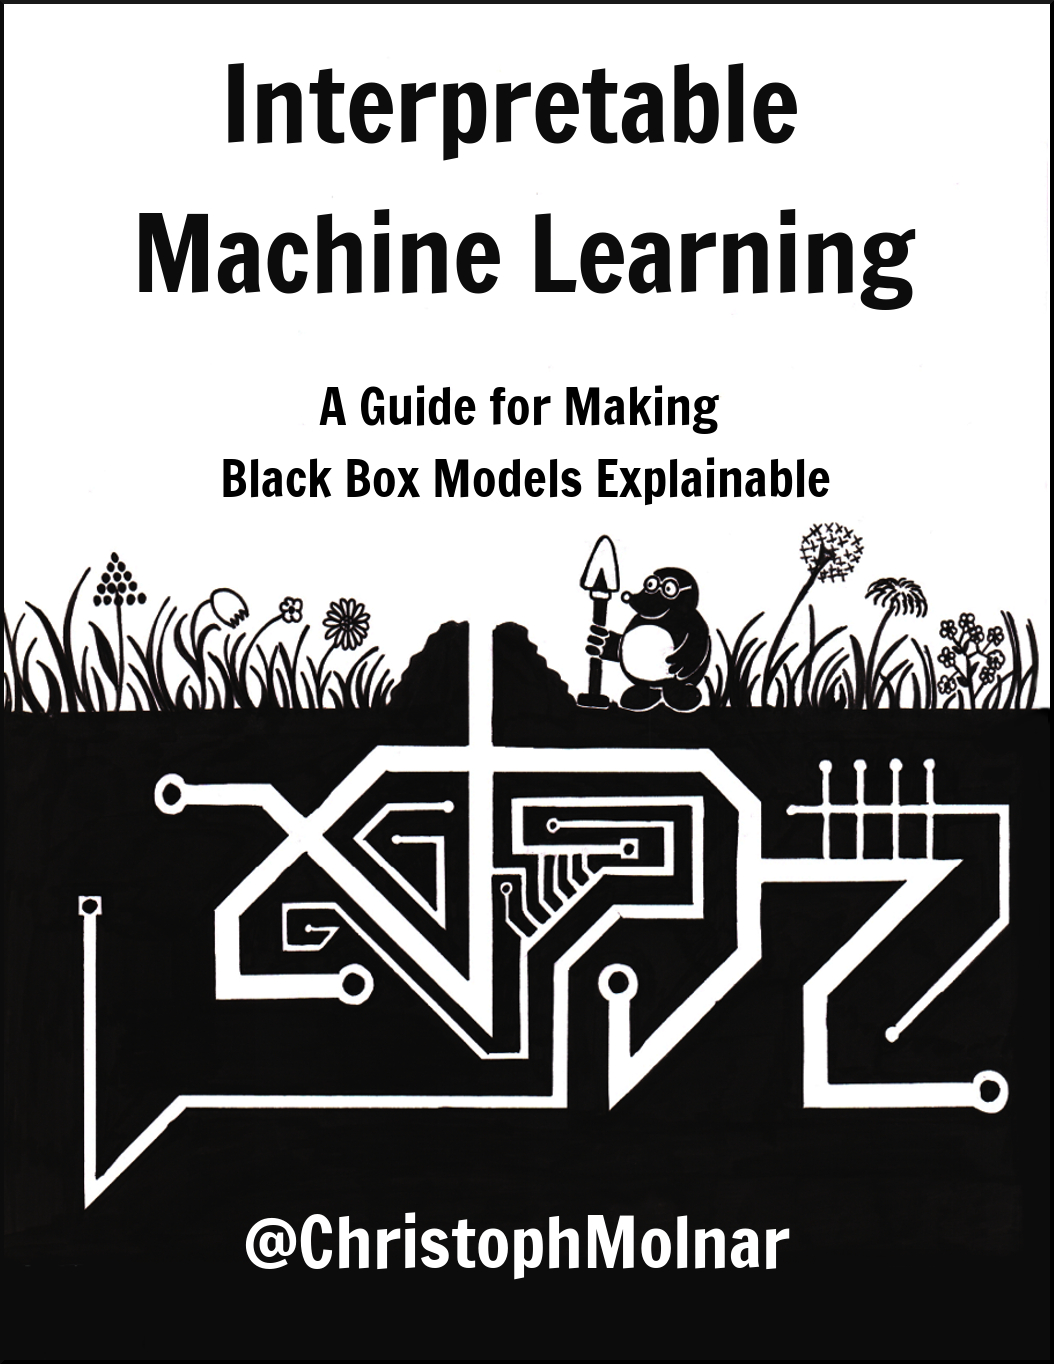
\includegraphics[scale=0.8]{images/title_page.jpg}
\end{figure*}

\chapter*{Lời nói đầu}
Machine learning (hay học máy) đã đạt được những thành tựu đáng kinh ngạc trong những năm vừa qua. 

Tuy máy tính có thể giúp con người thực hiện những tác vụ từ đơn giản tới phức tạp, tôi và bạn, những người đang học và làm việc với machine learning hầu như chỉ quan tâm tới kết quả hay dự đoán (prediction) của mô hình mà không chú ý tới quan hệ nhân quả (causality) trong học máy. Tại sao khi bạn đưa một bức ảnh của một chú mèo vào một mô hình \textbf{A}, giá trị trả về lại là ``\textit{cat}'' mà không phải là con vật khác? Có thể máy tính nhận diện được đôi tai hay con mắt, hay nó chỉ quan tâm tới hình dạng của vật thể? Tôi tin rằng, chỉ khi ta thực sự hiểu được mô hìn một cách cặn kẽ, ta mới có thể thực sự làm chủ trí tuệ nhân tạo (Artificial Intelligence - AI). Cuốn sách này được viết ra để giúp ta hiểu và giải thích cách thức hoạt động của các mô hình học máy.

Sau khi thống nhất định nghĩa về tính khả diễn giải hay khả giải thích (interpretability), ta sẽ đi vào tìm hiểu các mô hình khả diễn giải (interpretable models) như cây quyết định (decision trees), luật quyết định (decision rules), và hồi quy tuyến tính (linear regression). Tiếp theo đó ta tìm hiểu các phương pháp để giải thích các kết quả trả về của các mô hình có dạng hộp đen (black-box) trong học máy.

Cuốn sách này được dịch nhằm mục đích giúp các bạn đang học, làm việc, hoặc có sở thích tìm hiểu về học máy có cái nhìn tổng quan về một nhánh rất thú vị của học máy cũng như nắm bắt sơ bộ về cách thức hoạt động của các mô hình học máy hiện hành.  

Một động lực rất lớn khi dịch cuốn cách này của tôi đó là cộng đồng học Machine Learning ở Việt Nam đang chủ yếu chỉ tập trung vào Deep Learning (học sâu) mà bỏ qua những nhánh rất hay của Machine Learning, có thể kể ra như Continual Learning (học liên tục), Efficient Deep Learning (học sâu hiệu quả), Deep Generative Models (mô hình sinh sâu), hay Reinforcement Learning (học củng cố) vân vân. Theo tôi thấy, Deep Learning thực sự rất phù hợp với những bạn mới tiếp xúc với Machine Learning hoặc có mục đích đi làm. Nhưng với những bạn muốn đi học lên cao hoặc đi theo con đường nghiên cứu, việc đào sâu và tìm hiểu các mảng khác sẽ giúp các bạn có được khả năng viết những công trình khoa học và mở rộng tầm nhìn tới con đường khám phá tri thức khoa học phía trước. Với bản dịch này, tôi hi vọng có thể đóng góp một phần nhỏ bé giúp cộng đồng học Machine Learning ở Việt Nam lớn mạnh hơn bằng cách giới thiệu một hướng đi mới: học máy khả diễn giải (Interpretable Machine Learning). Mọi tài liệu liên quan đến bản dịch này được lưu trữ qua Github ở \href{https://github.com/giangnguyen2412/InterpretableMLBook-Vietnamese}{đây}.
